\setAuthor{Tundmatu autor}
\setRound{lahtine}
\setYear{2008}
\setNumber{G 10}
\setDifficulty{9}
\setTopic{Termodünaamika}

\prob{Pooljuht}
Graafikul on antud pulgakujulise keraamilisest pooljuhist (nn. PTC takisti) soojendi materjali erijuhtivuse $\sigma$ (\si{1/(\ohm. m)}) sõltuvus temperatuurist $t$(\si{\degreeCelsius}). Erijuhtivuseks nimetatakse eritakistuse pöördväärtust. Leida, millise temperatuurini kuumeneb avatud ruumis paiknev sellest materjalist soojendi, kui tema otstele rakendatakse pinge $U_1 = \SI{60}{V}$. Milliseks kujuneb soojendi temperatuur, kui otstele rakendatud pinge on $U_2 = \SI{36}{V}$? On teada, et kui soojendi otstele rakendatakse pinge $U_0 = \SI{30}{V}$, siis soojendi temperatuuriks kujuneb $t_0= \SI{70}{\degreeCelsius}$. Välisõhu temperatuur on $t_v = \SI{20}{\degreeCelsius}$.

\begin{center}
	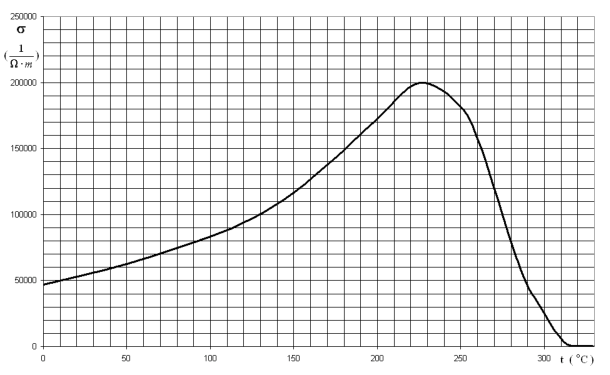
\includegraphics[width=\linewidth]{2008-lahg-10-yl}
\end{center}

\hint
Kütteelement on soojuslikus tasakaalus ümbritseva keskkonnaga ning kaod keskkonda on võrdelised sise- ja välistemperatuuride vahega. Soojusliku tasakaalu temperatuur on määratav nn graafilise meetodiga, mis seisneb $\sigma (t)$ ja teatud funktsiooni pingest lõikepunkti leidmises.

\solu
Kütteelemendi takistus on
\[
R=\frac{\rho L}{S}=\frac{L}{\sigma S},
\]
kus $\rho$ on eritakistus, $L$ elemendi pikkus, $S$ elemendi ristlõikepindala ja $\sigma$ erijuhtivus. Elemendil eralduv võimsus on
\[
N=\frac{U^{2}}{R}=\frac{S}{L} U^{2} \sigma.
\]
Võimsus, millega keha annab soojust ümbritsevale keskkonnale, on võrdeline temperatuuride vahega ja tasakaalulise temperatuuri puhul peab võrduma kehal eralduva võimsusega. Seega
\[
N=k \Delta t=\frac{S}{L} U^{2} \sigma.
\]
Siit näeme, et
\begin{equation} \label{2008-lahg-10:eq1}
\frac{\sigma}{\Delta t} \cdot U^{2}=k \frac{L}{S}=\const,
\end{equation}
kus aga $\frac{\sigma}{\Delta t}$
on sirge tõus erijuhtivuse graafikul, kus algpunktiks on $t_v = \SI{20}{\degreeCelsius}$ ja
$\sigma = \num{0}$.

\begin{center}
	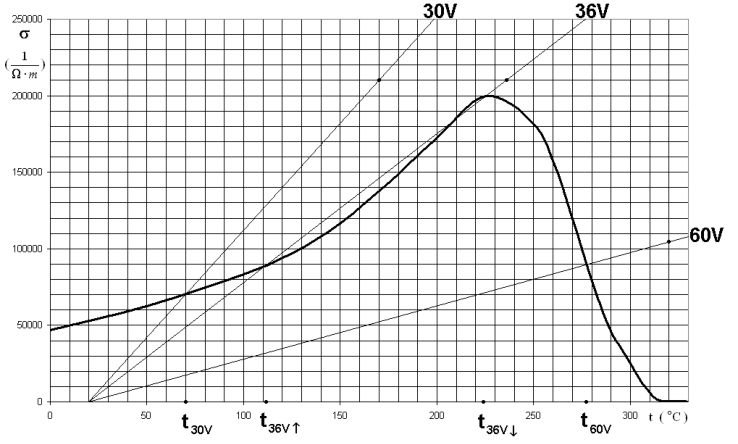
\includegraphics[width=\linewidth]{2008-lahg-10-lah}
\end{center}

Algtingimusi silmas pidades on pinge $U_0 = \SI{30}{V}$ juures see tõus $\left(\frac{\sigma}{\Delta t}\right)_{30}=\frac{7}{5}$ ning arvestades valemit (\ref{2008-lahg-10:eq1}) saame
\[
\left(\frac{\sigma}{\Delta t}\right)_{30} \cdot U_{0}^{2}=\left(\frac{\sigma}{\Delta t}\right)_{60} \cdot U_{1}^{2}=\left(\frac{\sigma}{\Delta t}\right)_{36} \cdot U_{2}^{2}.
\]
Siit 
\[
\begin{aligned}\left(\frac{\sigma}{\Delta t}\right)_{60} &=\frac{U_{0}^{2}}{U_{1}^{2}}\left(\frac{\sigma}{\Delta t}\right)_{30}=\frac{7}{20}, \\\left(\frac{\sigma}{\Delta t}\right)_{36} &=\frac{U_{0}^{2}}{U_{2}^{2}}\left(\frac{\sigma}{\Delta t}\right)_{30}=\frac{35}{36}. \end{aligned}
\]
Kanname vastavad sirged (alguspunktiga $t = \SI{20}{\degreeCelsius}$ ja $\sigma = 0$) graafikule ja loeme vastavad tasakaalulised temperatuurid.

Saame $U_1 = \SI{60}{V}$ puhul $t_1 = \SI{277}{\degreeCelsius}$.

Tekib huvitav nähtus, et tänu mittelineaarsusele on $U_2 = \SI{36}{V}$ puhul pinge tõstmisel ja langetamisel tasakaalulised temperatuurid erinevad, vastavalt pinge tõusul $t_2 = \SI{112}{\degreeCelsius}$ ja langetamisel $t_2' = \SI{224}{\degreeCelsius}$.

Paneme tähele, \SI{36}{V} puhul on graafikult loetavaid lahendeid justkui kolm, aga keskmine lahend \SI{207}{\degreeCelsius} on ebastabiilne. Nimelt olukorras, kus küttekeha on sellel temperatuuril, viib väikenegi küttekeha temperatuuri tõus võimsuse suurenemiseni ja langus vastavalt võimsuse vähenemiseni, ja seega temperatuur kas kasvab temperatuurini \SI{224}{\degreeCelsius} või langeb temperatuurini \SI{112}{\degreeCelsius}.
\probend